\newpage
\chapter{Introduction}
Heavy duty transport can be seen as the backbone of today's economy: all commerce, from local retailers to big e-commerce brands, would not be possible without it. It's one of the most important links of the logistics chain, given that it makes possible to have the capillarity and the short lead times to which we are all used in today's world.
But times like the ones we are living in oblige us to pose an important question: \textbf{\textit{is all this sustainable?}}

Given the report from ACEA\textsuperscript{\cite{ACEA2021}}, we can see that the circulating heavy duty fleets in EU have an average age of $13$ years, with a predominance of diesel powered vehicles (Figure \ref{fig:hdpower}).

\begin{figure}[hb]
    \centering
    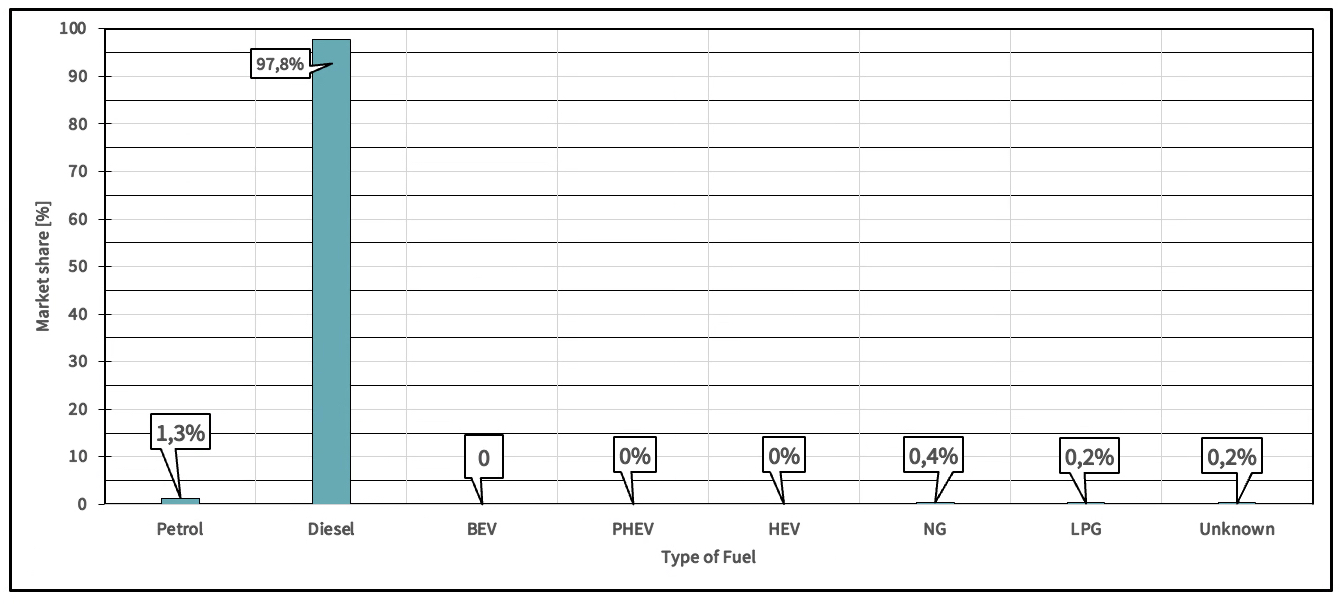
\includegraphics[width=0.7\textwidth]{Chapters/Pictures/Fuels_MarketShare.jpeg}
    \caption{Market share (in percentage) for different types of fuel}
    \label{fig:hdpower}
\end{figure}
The goods transportation sector has a prevailing weight on the energetic consumption of the European Union: in fact, over $40\%$ of all the liquid fuels for road use are consumed by this sector\textsuperscript{\cite{pianoidrogeno}}. So, in compliance with the UN sustainable development goals, the  necessity to renew this field is evident. How to do this is an interesting question that puts on the table different solutions, ranging from hybrid trucks coupled with overhead contact lines to be powered with when on highways, to "simple" battery electric trucks and passing also from $H_2$ solutions. In Table \ref{tab:dieselalternative} we can find the main options that can help us achieve this objective.

\newpage
\begin{table}[ht]
\centering
\begin{tabular}{|c|c|c|}
\hline
\rowcolor{bluepoli!40} \multicolumn{1}{|c|}{\textbf{Fuel}} & \multicolumn{1}{c|}{\textbf{PROS}}         & \multicolumn{1}{c|}{\textbf{CONS}} \\ \hline
\textbf{Biofuels} & Derivable from waste products & Still emit $CO_2$ during use \\ \hline
\textbf{Electricity} & \begin{tabular}[c]{@{}c@{}}$100\%$ clean during use; \\ Possible to couple the vehicle \\ with a fixed infrastructure \\ (OVH contact line)\end{tabular} & \begin{tabular}[c]{@{}c@{}}Cleanness depend on energetic mix; \\ Charging infrastructure and time \\ Weight of the battery\end{tabular} \\ \hline
\textbf{Hydrogen} & \begin{tabular}[c]{@{}c@{}}$100\%$ clean during use; \\ Higher energy density\end{tabular} & Lower volumetric density \\ \hline
\end{tabular}
\caption{Pros and Cons of different alternative fuels}
\label{tab:dieselalternative}
\end{table}

Regarding the use of batteries, as stated in a recent book by Professor R. Mazzoncini\textsuperscript{\cite{Mazzo2021}}, this is not so convenient, because of their size and type of use: to maintain a range which is compatible with a diesel solution, a BEV would weigh almost $5$ tons more. Hence, the focus to produce HD vehicles that are green during use needs to pass from $H_2$ technologies, which will be the focus of this paper.

\section{State of the Art}
The field of hydrogen production is in continuous development. In the recent years, more and more attention is being put in these technologies, as they can offer a solution to a handful of problems, starting from their being a cleaner solution for transportation sector. The actual production technologies are the following\textsuperscript{\cite{guanda20211}}:

\begin{description}
    \item[Oil:] hydrogen is produced with steam reforming or partial oxidation from fossil or renewable oils;
    \item[Gas:] natural or bio-gas can be used to produce hydrogen via steam reforming or partial oxidation;
    \item[Algae:] methods for utilising the photo-synthesis for hydrogen production;
    \item[Wood:] pyrolysis technology can be used for deriving hydrogen from biomass;
    \item[Electricity:] water electrolysis using electric power from renewable sources;
    \item[Coal:] with gasification technology hydrogen may be produced from coal;
    \item[Alcohols:] like hydrogen and methanol derived from gas or biomass (rich in hydrogen and may be reformed to hydrogen).
\end{description}

The technology we chose to deepen is \textit{electrolysis}, due to the good scalability of the plants, that range from few kW to several MW.

Due to the physical and geographical characteristics of Italy and the very virtuous energetic mix, in which almost $40\%$ of electric power comes from renewable sources, we chose to feed the water electrolysis with renewable energy. Namely, the two solutions we considered will be hydroeletctric plants and photovoltaic plants. Both these solutions also address the problem of being independent from the foreign states. This theme, which is really important, started to spread in the last years in the case of oil and gas, with few countries controlling their extraction and production.

\subsection{Electrolysis}
With electrolysis water is split in hydrogen and oxygen, in an electrochemical cell. A distinction can be made based on the cell's temperature\textsuperscript{\cite{guanda20211}}:

\begin{itemize}
    \item Low temperature cells that can be divided into:
    \begin{itemize}
        \item Alkaline electrolysis (Figure \ref{fig:alkaline})  based on a liquid solution of $NaOH$ or $KOH$;
        \item PEM (Figure \ref{fig:pem}) based on a polymeric electrolyte.
    \end{itemize}
    \item High temperature cells (such as SOEC).
\end{itemize}

Low temperature cells are already a commercial solution, while high temperature ones are still in development; hence, our focus will be on the former.

\subsection{Hydroelectric Energy}
Hydroelectric power plants use the potential energy of water flowing down into the turbine to produce electrical energy. We can find two main configurations\textsuperscript{\cite{lakohydro2010}}:

\begin{itemize}
    \item Dams with reservoirs (Figure \ref{fig:dam}), that can be classified into:
    \begin{itemize}
        \item Small dams;
        \item Large dams;
        \item Pumped storage;
    \end{itemize}
    \item Run-of-the-river.
\end{itemize}

This technology does not produce significant $CO_2$ emissions other than those emitted during the plant construction. It has also reached a significant degree of maturity: many of the plants that were built in the early decades of the $20^{th}$ century are currently still in operation. This reduces the costs of the facilities, because they consist simply in O$\&$M.

\begin{figure}[p]
    \centering
    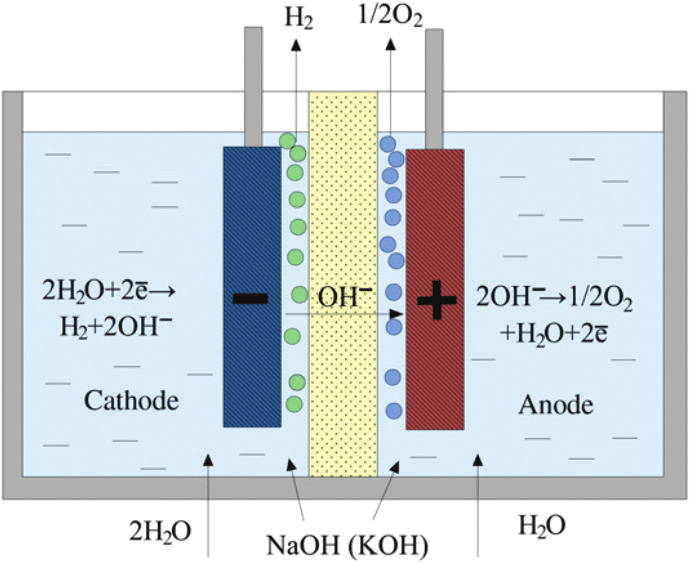
\includegraphics[width=0.5\textwidth]{Chapters/Pictures/Schematic-diagram-of-the-alkaline-electrolysis-cell-34.png}
    \caption{Schematic diagram of the alkaline electrolysis cell\textsuperscript{\cite{schemepictureelectrolysis}}}
    \label{fig:alkaline}
\end{figure}

\begin{figure}[p]
    \centering
    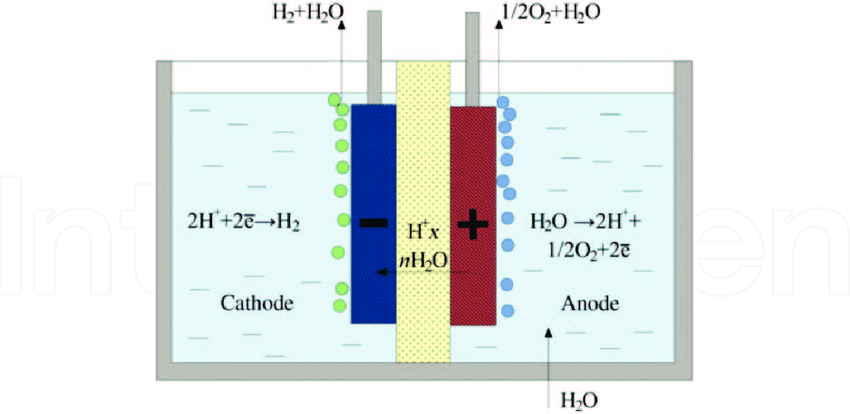
\includegraphics[width=0.8\textwidth]{Chapters/Pictures/Schematic-diagram-of-PEM-electrolysis-cell-33.png}
    \caption{Schematic diagram of PEM electrolysis cell\textsuperscript{\cite{schemepictureelectrolysis}}}
    \label{fig:pem}
\end{figure}

\begin{figure}[p]
    \centering
    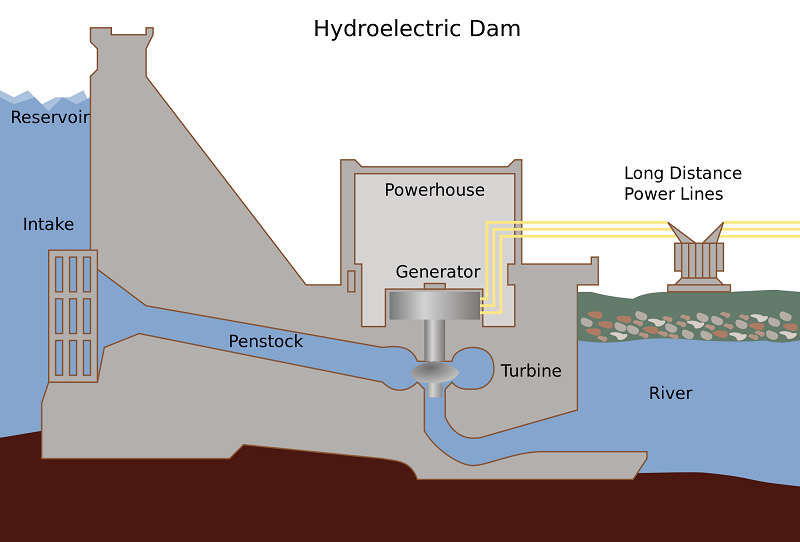
\includegraphics[width=0.5\textwidth]{Chapters/Pictures/Damparts.png}
    \caption{\small{A diagram showing the main components of a conventional hydroelectric facility\textsuperscript{\cite{hydropowerscheme}}}}
    \label{fig:dam}
\end{figure}

Otherwise hydropower depends on rainfall and a reserve may be needed to compensate for periods of low rainfall. So, it will be possible that climate change influences the efficiency of such technology. We also have to take in account the political, societal and economic risk usual of this type of infrastructures.

\subsection{Photovoltaic Energy}
The goal of a photovoltaic plant is to convert solar energy into electricity. To do that, a solar cell needs two main mechanisms\textsuperscript{\cite{PV2020}}:

\begin{enumerate}
    \item the light should be absorbed and electrons and holes should be generated in the conduction and valence band, respectively;
    \item the generated electrons and holes should be separated and transported to their selective contact.
\end{enumerate}

More in detail (Figure \ref{fig:pv}), the light is absorbed in the Light Absorbing Layer (the photon have higher energy of the LAL energy gap) and generate electrons and holes that will diffuse in the layer. If an electron reaches the interface between LOL and the Electron Selective Layer (ESL) it is into ESL and can reach the electrode. On the opposite, if an electron reaches the LAL and Hole Selective Layer (HSL), the gap prevents the charge transfer and reflect back the electron. The same thing happens for holes that are forced to move towards the positive electrode.

\begin{figure}[h]
    \centering
    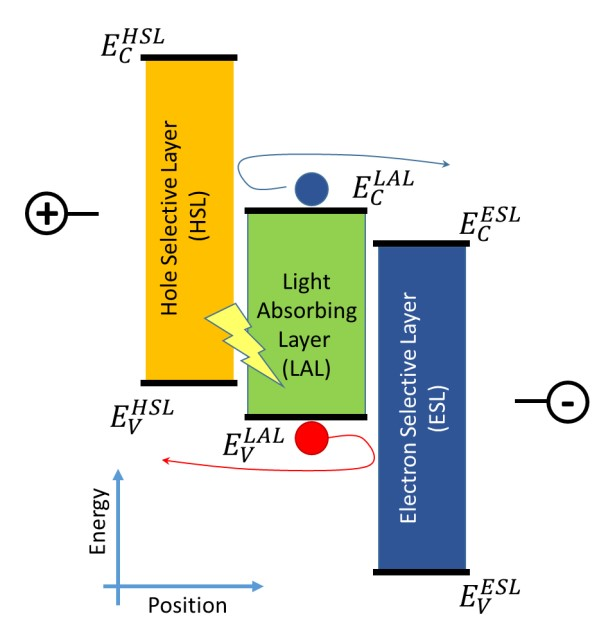
\includegraphics[width=0.5\textwidth]{Chapters/Pictures/PV_schematic_diagram.jpg}
    \caption{Schematic diagram of key elements for solar cells\textsuperscript{\cite{PV2020}}}
    \label{fig:pv}
\end{figure}
\newpage
There are various generations of photovoltaic panels, that can be classified into two categories:

\begin{description}
    \item[Wafer-based cells] are fabricated on semiconducting wafers and can be handled without an additional substrate, although modules are typically covered with glass for mechanical stability and protection;
    \item[Thin-film cells]  consist of semiconducting films deposited onto a glass, plastic, or metal substrate. We can divide them into commercial and emerging thin-film technologies.
\end{description}

We can also say\textsuperscript{\cite{PV2020}} that PV can adapt to the application requests by varying aspect and will spread in different sector but, at the same time, its future is still open for strong innovations with the aims to reach the maximum efficiency of $95\%$ instead of the present record of $47,1\%$.

\section{Example Project}

The creation of a grid of hydrogen refilling station is a great challenge that is going to require, in the near future, some great advancements in the field. 

Regarding Italy, the actual $H_2$ refilling infrastructure is still way behind the level needed for a mass diffusion of this technology. Only one station is actually active, and a lot of them are still under development.

One virtuous example is \textit{$H_2$ SUDTIROL}\textsuperscript{\cite{centroidrogenobolzano}}.

$H_2$ Sudtirol is a site located in Bolzano, where green hydrogen is produced locally by means of electrolysis powered by renewable energy. The main goal of this project was to find a way to store the surplus of clean energy provided by hydroelectric power plants in the form of hydrogen. The modular electrolysers on site are able to produce up to $180$ Nm\textsubscript{3}/hour. The hydrogen is than compressed and stored and can refill up to $15$ urban buses (with $200/250$ km of range) or up to $700$ cars.